% Template for white paper submissions for the 
% LSST Call for Observing Strategies for DeepDrilling and Minisurveys 
% 
% The call for white papers can be found at https://github.com/lsst-pst/survey_strategy/blob/master/latex/WPcall2018.pdf
% The deadline for submissions is November 29, 2018
% Please submit your white paper via a pull request at https://github.com/lsst-pst/survey_strategy_wp, after creating a 
%   subdirectory named LASTNAME_FIRSTNAME_NUMBER
% For help with white papers or the submission process, please post at http://community.lsst.org/c/sci/survey-strategy


\documentclass[11pt]{article}
\usepackage[utf8]{inputenc}
\usepackage{booktabs}
\usepackage{hyperref}
\usepackage{graphicx}

\title{Example White Paper Submitted in support of Target of Opportunity style Observations}
\author{Lynne Jones}
\date{April 2018}

\begin{document}

\maketitle

\begin{abstract}
A real white paper would have a short summary of the science case and modification to the survey strategy
here. Since this is not a real white paper, but an example, that will be lacking here. The general idea of this
example, however, is to show how this template might be filled in. 
\end{abstract}

\section{White Paper Information}
Please contact Lynne Jones, University of Washington, lynnej@uw.edu, with any questions about this white paper. 

This white paper addresses:
\begin{itemize} 
\item an integrated program with science that hinges on the combination of pointing/detailed 
	observing strategy combination. 
\end{itemize}  

\clearpage

\section{Scientific Motivation}

\begin{footnotesize}
{\it Describe the scientific justification for this white paper in the context
of your field, as well as the importance to the general program of astronomy. 
(Limit: 2 pages + 1 page for figures/references.)}
\end{footnotesize}

Again, example white paper here, not a real white paper. But for the purposes of this
example, we're pretending that there is some kind of transient that is not well localized
by whatever gives us the alert that the transient is occurring (maybe it's gravitational waves 
and we're looking for optical counterparts?).  By finding the optical counterparts of
these objects discovered via very different techniques, we will be able to learn 
several amazing things that will help us learn about our area of astronomy. This will 
also provide links between several different areas of astronomy. This will be incredible. 
Given some theoretical models or perhaps previous empirical evidence, we expect to have 6 good ToO triggers per year. 
Even if we only find a single counterpart, we can learn these amazing things.
Great, I have explained why this is important.  Perhaps I put in a couple of figures showing why it's so awesome.

Of course, we should also mention why LSST is important for this science. LSST could be used 
to do many things, but ideally the science/survey strategy being discussed is a well matched with LSST's particular
capabilities. 

So for example's sake, let's say it's because the alert does provide localization of about 50 deg$^2$, or a circle with 
a diameter of about 8 degrees. The optical counterpart could be anywhere within this area, and we don't really know its
expected brightness but given that other surveys haven't already found these counterparts, it's probably fainter than $r=21$. 
The LSST field of view is about 3.5 deg across, and we could cover the area suggested by the alert with about 7 pointings
(see Figure~\ref{fig:tiling}).  The combination of large field of view and faint limiting magnitude provide the opportunity
to rapidly discover these optical counterparts, in a way we couldn't with other telescopes. 
Followup after localization of the optical counterpart would be done by other telescopes, once the large field of view
of LSST is not necessary.


\begin{figure}
\centering
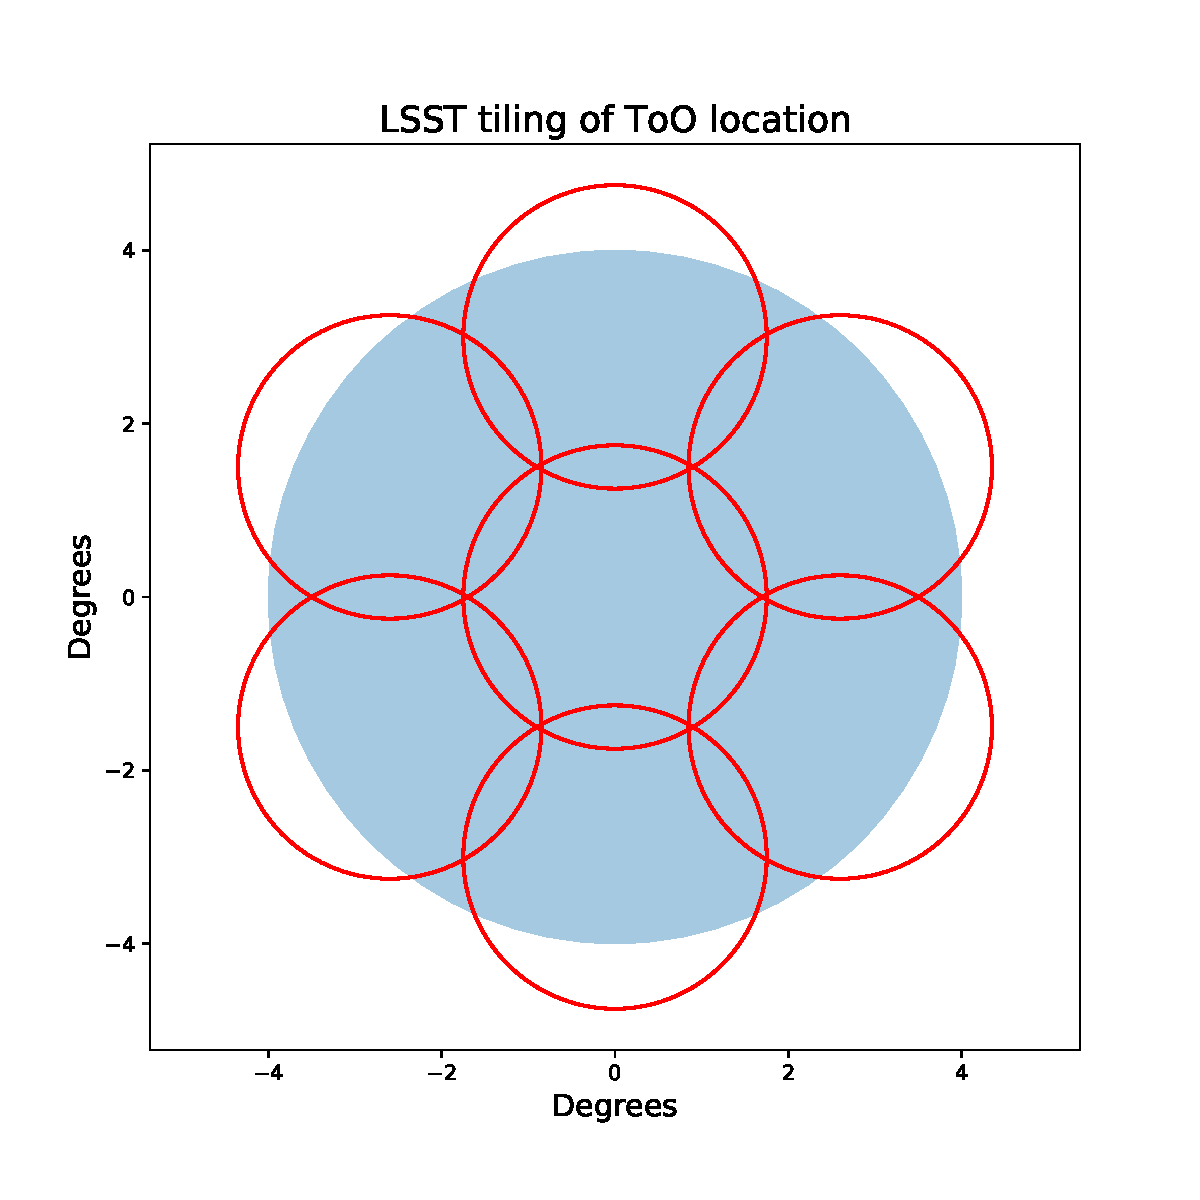
\includegraphics[width=0.5\textwidth]{ToO_tiling}
\caption{Example of tiling a ToO target with several LSST fields. You could definitely improve this by using the actual LSST footprint,
or a better approximation of the footprint. But this does give the general idea. \label{fig:tiling}}
\end{figure}

\clearpage

\section{Technical Description}
\begin{footnotesize}
{\it Describe your proposed observations. Please comment on each observing constraint
below, including the technical motivation behind any constraints. Where relevant, indicate
if the constraint applies to all requested observations or a specific subset. Please note which 
constraints are not relevant or important for your science goals.}
\end{footnotesize}

\subsection{High-level description}
\begin{footnotesize}
{\it Describe or illustrate your ideal sequence of observations.}
\end{footnotesize}

In our hypothetical example, we expect about 12 ToO events per year, 6 of which would be suitable targets for LSST (in the right hemisphere, 
having the right expected optical magnitude, etc.). These events would be relatively evenly spread throughout 
the year. For each event, we would tile an area of about 50 deg$^2$ around
the best predicted RA/Dec, with a pattern similar to that shown in Figure~\ref{fig:tiling}. We would like to cover
the tiling with a sequence of visits in $r$ band (all pointings), then $u$ band, followed by $y$ band for colors (thus, 7 visits in
$r$, 7 in $u$ and 7 in $y$).  We would follow this with an additional round of observations in $r$ band, to reject moving objects
and gain a better understanding of other transients in the field. This final round of $r$ band visits must be obtained within 24 hours
(or some other timescale that would be suitable for the expected fading of the ToO).  

In the each year, each visit would match the typical main survey visit time of 30 seconds to achieve a similar depth to the reference catalogs
and to allow standard LSST difference image processing to be used to identify transients. 
if the $y$ band filter is not available, $z$ band should be substituted. If $u$ band is not available, $g$ should be substituted.

\subsection{Footprint -- pointings, regions and/or constraints}
\begin{footnotesize}{\it Describe the specific pointings or general region (RA/Dec, Galactic longitude/latitude or 
Ecliptic longitude/latitude) for the observations. Please describe any additional requirements, especially if there
are no specific constraints on the pointings (e.g. stellar density, galactic dust extinction).}
\end{footnotesize}

The pointings will be determined by the location of the events. For purposes of simulating these events,
pointings spread randomly over the sky are sufficient. 

\subsection{Image quality}
\begin{footnotesize}{\it Constraints on the image quality (seeing).}\end{footnotesize}

No constraints on image quality.

\subsection{Individual image depth and/or sky brightness}
\begin{footnotesize}{\it Constraints on the sky brightness in each image and/or individual image depth for point sources.
Please differentiate between motivation for a desired sky brightness or individual image depth (as 
calculated for point sources). Please provide sky brightness or image depth constraints per filter.}
\end{footnotesize}

No constraints on individual image depth. 

\subsection{Co-added image depth and/or total number of visits}
\begin{footnotesize}{\it  Constraints on the total co-added depth and/or total number of visits.
Please differentiate between motivations for a given co-added depth and total number of visits. 
Please provide desired co-added depth and/or total number of visits per filter, if relevant.}
\end{footnotesize}

No constraints on coadded image depth or total number of visits.

\subsection{Number of visits within a night}
\begin{footnotesize}{\it Constraints on the number of exposures (or visits) in a night, especially if considering sequences of visits.  }
\end{footnotesize}

Ideally would obtain sequences of $r$, $u$, $y$, $r$ over the tiling in each night. If later sequences are interrupted, a
followup sequence of observations in $r$ as soon as possible (within 24 hours) would be necessary. 

\subsection{Distribution of visits over time}
\begin{footnotesize}{\it Constraints on the timing of visits --- within a night, between nights, between seasons or
between years (which could be relevant for rolling cadence choices in the WideFastDeep. 
Please describe optimum visit timing as well as acceptable limits on visit timing, and options in
case of missed visits (due to weather, etc.). If this timing should include particular sequences
of filters, please describe.}
\end{footnotesize}

The visits within the night must be sequential; covering the tiling pattern once in $r$, then in $u$, then in $y$ and then $r$ again.

\subsection{Filter choices}
\begin{footnotesize}
{\it Please describe any special filter requests not included above.}
\end{footnotesize}

\subsection{Exposure constraints}
\begin{footnotesize}
{\it Describe any constraints on the minimum or maximum exposure time required (or alternatively, saturation limits).
Please comment on any constraints on the number of exposures in a visit.}
\end{footnotesize}

Exposure constraints are based on estimates of the depth of the comparison catalog available, and are intended to
reach as faint a limiting magnitude possible while still having catalog data to identify transients.

\subsection{Other constraints}
\begin{footnotesize}
{\it Any other constraints.}
\end{footnotesize}

\subsection{Estimated time requirement}
\begin{footnotesize}
{\it Approximate total time requested for these observations, using the guidelines available at \url{https://github.com/lsst-pst/survey_strategy_wp}.}
\end{footnotesize}

Each event trigger would require:
\begin{itemize}
\item Slew to the first field and change filter to $r$ if necessary: simultaneous slew and filter change (120 seconds) 
\item Visits across all 7 pointings in the tiling, in $r$ band. Time required is (30 seconds + 3 seconds slew/settle + 2 seconds shutter open/close) * 7 =  245 seconds
\item Change filter to $u$ band: 120 seconds 
\item Repeat the previous steps for observing in $u$ band (245 seconds)
\item Change to $y$ filter (120 seconds), 
\item Repeat observing in $y$ (245 seconds)
\item Change filter to $r$ band (120 seconds)
\item Repeat observing in $r$ (245 seconds)
\item Returning the LSST system to its previous state: simultaneous slew and filter change (120 seconds)
\end{itemize}
for a time requirement of 1580 seconds (26 minutes) per event. We estimate there will be about 6 events triggered in a year, for a total time requirement of 9480 seconds (2.6 hours) per year.

Over all 10 years of LSST, responding to these ToOs would require about 26.3 hours, less than 1\% of the total time available. 

\begin{table}[ht]
    \centering
    \begin{tabular}{l|l|l|l}
        \toprule
        Properties & Importance \hspace{.3in} \\
        \midrule
        Image quality &  2   \\
        Sky brightness &  1\\
        Individual image depth & 2  \\
        Co-added image depth &  1 \\
        Number of exposures in a visit   & 1  \\
        Number of visits (in a night)  &   1\\ 
        Total number of visits &  1 \\
        Time between visits (in a night) &  3\\
        Time between visits (between nights)  &  1 \\
        Long-term gaps between visits &1 \\
        Filters used in visits & 3 \\
        Timeliness of response to trigger & 3\\
        \bottomrule
    \end{tabular}
    \caption{{\bf Constraint Rankings:} Summary of the relative importance of various survey strategy constraints. Please rank the importance of each of these considerations, from 1=very important, 2=somewhat important, 3=not important. If a given constraint depends on other parameters in the table, but these other parameters are not important in themselves, please only mark the final constraint as important. For example, individual image depth depends on image quality, sky brightness, and number of exposures in a visit; if your science depends on the individual image depth but not directly on the other parameters, individual image depth would be `1' and the other parameters could be marked as `3', giving us the most flexibility when determining the composition of a visit, for example.}
        \label{tab:obs_constraints}
\end{table}

\subsection{Technical trades}
\begin{footnotesize}
{\it To aid in attempts to combine this proposed survey modification with others, please address the following questions:
\begin{enumerate}
    \item What is the effect of a trade-off between your requested survey footprint (area) and requested co-added depth or number of visits?
    \item If not requesting a specific timing of visits, what is the effect of a trade-off between the uniformity of observations and the frequency of observations in time? e.g. a `rolling cadence' increases the frequency of visits during a short time period at the cost of fewer visits the rest of the time, making the overall sampling less uniform.
    \item What is the effect of a trade-off on the exposure time and number of visits (e.g. increasing the individual image depth but decreasing the overall number of visits)?
    \item What is the effect of a trade-off between uniformity in number of visits and co-added depth? Is there any benefit to real-time exposure time optimization to obtain nearly constant single-visit limiting depth?
    \item Are there any other potential trade-offs to consider when attempting to balance this proposal with others which may have similar but slightly different requests?
\end{enumerate}}
\end{footnotesize}

There aren't really very many trades to consider with these suggested responses to ToOs. The observations have to happen quickly in response to the event trigger, and
at the location of the trigger. Changing the time sampling of the visits within the night is undesirable, because the sequence is intended to narrow down on the optical
colors. 

\section{Performance Evaluation}
\begin{footnotesize}
{\it Please describe how to evaluate the performance of a given survey in achieving your desired
science goals, ideally as a heuristic tied directly to the observing strategy (e.g. number of visits obtained
within a window of time with a specified set of filters) with a clear link to the resulting effect on science.
More complex metrics which more directly evaluate science output (e.g. number of eclipsing binaries successfully
identified as a result of a given survey) are also encouraged, preferably as a secondary metric.
If possible, provide threshold values for these metrics at which point your proposed science would be unsuccessful 
and where it reaches an ideal goal, or explain why this is not possible to quantify. While not necessary, 
if you have already transformed this into a MAF metric, please submit the code in addition to the text description. (Limit: 2 pages).}
\end{footnotesize}

The survey will achieve these goals if it obtains the full sequence of observations of the ToO trigger within a night of the trigger event. If $g$ or $z$ band filters 
have to be swapped for $u$ or $y$, then the sequence is still valid. If a partial sequence (missing some filters) is obtained, then the observations are still useful 
but with a reduced benefit. If only some sections of the tiling are obtained, the observations are still useful but at a lower level. 

Each trigger could be scored on a level of 0-7, with 7 for a perfect set of observations. For each field that receives a complete set of observations in all filters, add 1 to
the score. For each field that is observed in only some filters, add 1/3 * number of filters, as long as two visits are obtained in $r$ band (even if the second
$r$ band visits must be obtained several hours later). If a given trigger scores 5 or above, it is counted as ``successful''. Obtaining 
successful followup of at least 5 ToOs indicates good performance for this science, a reasonable threshold given the rarity of the events.

As an example: a trigger event occurred and LSST obtained observations at the required location in the same night (within an hour of the event, even). All 7 pointings 
within the tiling obtained observations in $r$ band. As it was not dark time, $u$ was not available so $g$ band was substituted. All 7 pointings obtained visits in $g$ 
band. Only 5 fields obtained visits in $y$ band, as the field set below the LSST pointing limits. None received a second round of $r$ band visits in the same night.
A second set of visits in $r$ were obtained as soon as it was visible in the next night; these were within the 24 hour cutoff. 
The total score for this event would be 5 + 2/3 * 2 = 6.3. This trigger is ``successful''.  

\section{Special Data Processing}
\begin{footnotesize}
{\it Describe any data processing requirements beyond the standard LSST Data Management pipelines and how these will be achieved.}
\end{footnotesize}

The data processing follows the same plan as standard LSST data processing -- difference imaging against standard LSST templates would identify potential optical counterparts, although a custom filter on the resulting alert stream would be required. This filter would require the potential counterparts to be present in
both sets of $r$ band images (to reject moving objects), and place some constraint on relative $r$ and $y$ color. 

\end{document}
